\documentclass{standalone}
\usepackage{amsmath}
\usepackage{graphicx}
\usepackage{overpic}
\usepackage{tikz}

\begin{document}

	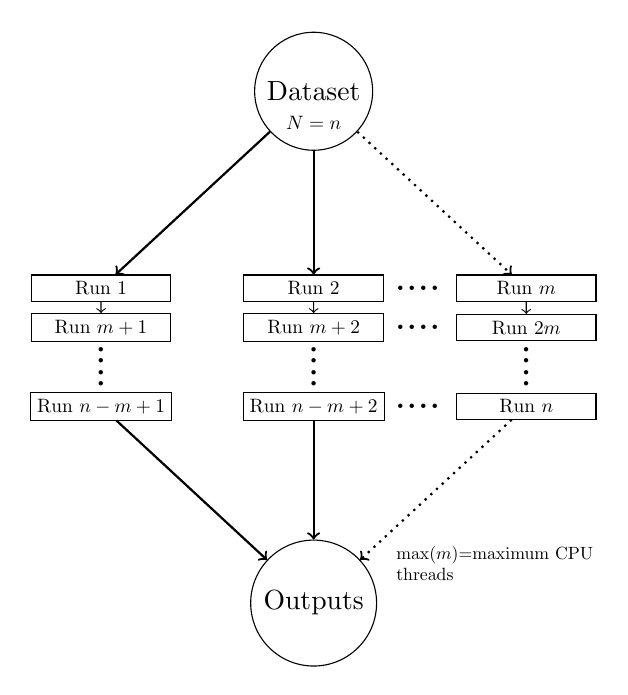
\begin{tikzpicture}
	\usetikzlibrary{graphs}
	\usetikzlibrary{backgrounds}
		\begin {scope} [on background layer]
		\node [ rectangle, fill=white,text width=200,text height=210] {};
		\end {scope}
		
	\node [name=master,draw,circle,black,scale=1] at (0,3) {Dataset};
	\node [scale=0.7] at (0,2.6) {$N=n$};
	
	\node [name=run1,draw, rectangle, black, scale=0.7,minimum width=72] at (-2.7,0.5) {Run 1};
	\node [name=run2,draw, rectangle, black, scale=0.7, minimum width=72] at (0,0.5) {Run 2};
	\node [name=runn,draw, rectangle, black, scale=0.7, minimum width=72] at (2.7,0.5) {Run $m$};
	
	
	\node [name=runn1,draw, rectangle, black, scale=0.7,minimum width=72] at (-2.7,0) {Run $m+1$};
	\node [name=runn2,draw, rectangle, black, scale=0.7,minimum width=72] at (0,0) {Run $m+2$};
	\node [name=runnn,draw, rectangle, black, scale=0.7, minimum width=72] at (2.7,0) {Run $2m$};
	
	\node [name=runnn1,draw, rectangle, black, scale=0.7] at (-2.7,-1) {Run $n-m+1$};
	\node [name=runnn2,draw, rectangle, black, scale=0.7] at (0,-1) {Run $n-m+2$};
	\node [name=runnnn,draw, rectangle, black, scale=0.7, minimum width=72] at (2.7,-1) {Run $n$};
	
	\node [name=output,draw, circle, black,scale=1] at (0,-3.5) {Outputs};
	
	\node[name=dots,scale=1.5] at (1.32,0.5) {....};
	\node[name=dots,scale=1.5] at (1.32,0) {....};
	\node[name=dots,scale=1.5] at (1.32,-1) {....};
	
	\node[name=dots,scale=1.5,rotate=90] at (-2.7,-0.5) {....};
	\node[name=dots,scale=1.5,rotate=90] at (0,-0.5) {....};
	\node[name=dots,scale=1.5,rotate=90] at (2.7,-0.5) {....};
	
	
	
	\node[scale=0.64,align=left] at (2.3,-3) {max$(m)$=maximum CPU\\threads};
%	\node [thick,scale=0.5, rotate=52] at (-1.35,0.5) {Sample 1};
%	\node [thick,scale=0.5, rotate=90] at (-0.15,0.5) {Sample 2};
%	\node [thick,scale=0.5, rotate=-52] at (1.02,0.5) {Sample $n$};
	
	
	
	
	
	\graph {(master)->[thick] {(run1),(run2)}};
	\graph {(master)-> [dotted,thick] (runn)};	
	\graph {(run1)->  (runn1)};
	\graph {(run2)->  (runn2)};
	\graph {(runn)->  (runnn)};
	
	\graph {(runnn1)-> [thick]  (output)};
	\graph {(runnn2)-> [thick](output)};
	\graph {(runnnn)-> [thick,dotted] (output)};


	\end{tikzpicture}
\end{document}